\documentclass[10pt,twocolumn]{article}
\usepackage[a4paper,margin=17mm,columnsep=6mm]{geometry}
\usepackage[T1]{fontenc}
\usepackage{newtxtext,newtxmath}
\usepackage{graphicx}
\usepackage{booktabs}
\usepackage{amsmath}
\usepackage[numbers,sort&compress]{natbib}
\usepackage[font=small,labelfont=bf,labelsep=period]{caption}
\usepackage{enumitem}
\usepackage{microtype}
\usepackage{xcolor}
\usepackage[colorlinks=true,linkcolor=black,citecolor=black,urlcolor=blue!50!black]{hyperref}
\setlist{nosep,leftmargin=1.2em}
\setlength{\bibsep}{1pt}
\setlength{\emergencystretch}{1.5em}
% Generated by scripts/export_compact_paper.py from results/; do not edit. Sources: numbers_sources.json
\newcommand{\SoneDstar}{62.9}
\newcommand{\SoneDstarFine}{48.9}
\newcommand{\SoneDstarExclLo}{5.4}
\newcommand{\SoneDstarExclHi}{6.9}
\newcommand{\SoneKTtwoDiff}{\ensuremath{-}0.005}
\newcommand{\SoneKTtwoDiffLo}{\ensuremath{-}0.012}
\newcommand{\SoneKTtwoDiffHi}{\ensuremath{-}0.003}
\newcommand{\SoneKTtwoPermP}{\ensuremath{\approx}\,0.38}
\newcommand{\SoneKTtwoGain}{0.022}
\newcommand{\SoneHoldGzero}{0.42}
\newcommand{\SoneRelGzero}{1.22}
\newcommand{\SoneHoldMax}{9.51}
\newcommand{\SoneCapGain}{0.7}
\newcommand{\SoneDaccGone}{\ensuremath{-}1.87}
\newcommand{\SoneDaccGoneLo}{\ensuremath{-}1.91}
\newcommand{\SoneDaccGoneHi}{\ensuremath{-}1.83}
\newcommand{\SoneDaccMin}{\ensuremath{-}18.7}
\newcommand{\SoneSMUnclamped}{\ensuremath{-}0.72}
\newcommand{\SoneSMRatio}{0.99}
\newcommand{\SoneEnvHold}{9.93}
\newcommand{\SoneEnvRel}{3.10}
\newcommand{\SoneEnvDacc}{\ensuremath{-}1.19}
\newcommand{\SoneEnvDaccLo}{\ensuremath{-}1.24}
\newcommand{\SoneEnvDaccHi}{\ensuremath{-}1.15}
\newcommand{\SoneEnvDaccPooled}{\ensuremath{-}1.48}
\newcommand{\SoneEnvHighGain}{53}
\newcommand{\SoneAUCRing}{0.623}
\newcommand{\SoneAUCSM}{0.631}
\newcommand{\SoneAUCAcc}{0.630}
\newcommand{\SoneAUCVote}{0.626}
\newcommand{\SoneAUCSum}{0.623}
\newcommand{\SoneAUCStatic}{0.624}
\newcommand{\SoneAUCRingLo}{0.612}
\newcommand{\SoneAUCRingHi}{0.632}
\newcommand{\SoneHoneDiff}{\ensuremath{-}0.0088}
\newcommand{\SoneHoneDiffLo}{\ensuremath{-}0.0157}
\newcommand{\SoneHoneDiffHi}{\ensuremath{-}0.0025}
\newcommand{\SoneHonePermP}{\ensuremath{\approx}\,0.003}
\newcommand{\SoneHoneSumP}{\ensuremath{\approx}\,0.003}
\newcommand{\SoneHoneStaticP}{\ensuremath{\approx}\,0.027}
\newcommand{\SoneNoDecoyLo}{0.643}
\newcommand{\SoneNoDecoyHi}{0.645}
\newcommand{\SoneDecoyRing}{0.491}
\newcommand{\SoneDecoySM}{0.552}
\newcommand{\SoneFalseSun}{0.12}
\newcommand{\SoneSpeed}{0.36}
\newcommand{\SoneCompass}{0.49}
\newcommand{\SoneThreeDGain}{0.022}
\newcommand{\SoneNoFaultRing}{0.98}
\newcommand{\SoneNmissions}{45{,}000}
\newcommand{\SoneHthreePeak}{3.25}
\newcommand{\SoneHthreePeakGain}{0.3}
\newcommand{\SoneHthreeCeil}{3.82}
\newcommand{\SoneUsableTwoD}{13}
\newcommand{\SoneUsableThreeD}{24}
\newcommand{\SoneHthreeAccGzero}{1.06}
\newcommand{\SoneHthreeAccGzeroLo}{0.44}
\newcommand{\SoneHthreeAccGzeroHi}{1.71}
\newcommand{\SoneHthreeStopGone}{0.00}
\newcommand{\SoneHthreeLimitGone}{0.99}
\newcommand{\SoneMB}{0.502}
\newcommand{\SoneMBLo}{0.494}
\newcommand{\SoneMBHi}{0.510}
\newcommand{\SonePix}{0.506}
\newcommand{\SoneDinoOff}{0.761}
\newcommand{\SoneDinoOn}{0.799}
\newcommand{\StwoHeadRing}{3.64}
\newcommand{\StwoHeadRingLo}{3.38}
\newcommand{\StwoHeadRingHi}{3.91}
\newcommand{\StwoHeadKF}{0.88}
\newcommand{\StwoHeadCF}{4.79}
\newcommand{\StwoHeadVone}{57.6}
\newcommand{\StwoHeadKFdiff}{\ensuremath{-}2.76}
\newcommand{\StwoHeadKFdiffLo}{\ensuremath{-}3.03}
\newcommand{\StwoHeadKFdiffHi}{\ensuremath{-}2.50}
\newcommand{\StwoCompassRing}{9.34}
\newcommand{\StwoCompassCF}{6.27}
\newcommand{\StwoCompassKF}{1.05}
\newcommand{\StwoKTsevenGated}{0.824}
\newcommand{\StwoKTsevenVote}{0.865}
\newcommand{\StwoKTsevenP}{\ensuremath{<}\,0.001}
\newcommand{\StwoSMtimeOff}{0.015}
\newcommand{\StwoTimeOffLo}{1.5}
\newcommand{\StwoTimeOffHi}{4.9}
\newcommand{\StwoTimeOffMid}{0.03}
\newcommand{\StwoTimeOffHigh}{0.66}
\newcommand{\StwoFront}{0.686}
\newcommand{\StwoFrontLo}{0.655}
\newcommand{\StwoFrontHi}{0.720}
\newcommand{\StwoMargin}{0.185}
\newcommand{\StwoMarginLo}{0.150}
\newcommand{\StwoMarginHi}{0.219}
\newcommand{\StwoNN}{0.732}
\newcommand{\StwoDino}{0.797}
\newcommand{\StwoMBvone}{0.501}
\newcommand{\StwoFrontNinety}{0.32}
\newcommand{\StwoMSvsGoal}{\ensuremath{-}0.019}
\newcommand{\StwoMSvsGoalLo}{\ensuremath{-}0.059}
\newcommand{\StwoMSvsGoalHi}{0.024}
\newcommand{\Nseeds}{300}
\newcommand{\StwoNmissions}{127{,}500}
\newcommand{\StwoNarms}{17}
\newcommand{\StwoNoFault}{0.990}
\newcommand{\StwoNoFaultLo}{0.971}
\newcommand{\StwoNoFaultHi}{0.997}
\newcommand{\StwoAUC}{0.852}
\newcommand{\StwoAUCLo}{0.840}
\newcommand{\StwoAUCHi}{0.863}
\newcommand{\StwoAUCvone}{0.009}
\newcommand{\StwoDiffVone}{0.843}
\newcommand{\StwoDiffVoneLo}{0.831}
\newcommand{\StwoDiffVoneHi}{0.855}
\newcommand{\StwoVoneOwn}{0.627}
\newcommand{\StwoDiffOwn}{0.225}
\newcommand{\StwoDiffOwnLo}{0.212}
\newcommand{\StwoDiffOwnHi}{0.239}
\newcommand{\StwoMidOcc}{0.95}
\newcommand{\StwoMidDecoy}{0.39}
\newcommand{\StwoMidCompass}{0.86}
\newcommand{\StwoMidEye}{0.81}
\newcommand{\StwoMidSun}{0.98}
\newcommand{\StwoMidSpeed}{0.98}
\newcommand{\StwoMidGust}{0.71}
\newcommand{\StwoMidMin}{0.71}
\newcommand{\StwoDecoyLo}{0.34}
\newcommand{\StwoDecoyHi}{0.40}
\newcommand{\StwoAblLanding}{0.849}
\newcommand{\StwoAblLandingLo}{0.837}
\newcommand{\StwoAblLandingHi}{0.860}
\newcommand{\StwoAblHome}{0.645}
\newcommand{\StwoAblHomeLo}{0.622}
\newcommand{\StwoAblHomeHi}{0.669}
\newcommand{\StwoAblHeading}{0.110}
\newcommand{\StwoAblHeadingLo}{0.100}
\newcommand{\StwoAblHeadingHi}{0.118}
\newcommand{\StwoAblFront}{0.030}
\newcommand{\StwoAblFrontLo}{0.019}
\newcommand{\StwoAblFrontHi}{0.040}
\newcommand{\StwoAblGated}{0.020}
\newcommand{\StwoAblGatedLo}{0.010}
\newcommand{\StwoAblGatedHi}{0.030}
\newcommand{\StwoAblInspect}{\ensuremath{-}0.004}
\newcommand{\StwoAblInspectLo}{\ensuremath{-}0.012}
\newcommand{\StwoAblInspectHi}{0.002}
\newcommand{\StwoMinusHomeAUC}{0.207}
\newcommand{\StwoMinusHeadingAUC}{0.742}
\newcommand{\StwoKF}{0.805}
\newcommand{\StwoRingMinusKF}{0.047}
\newcommand{\StwoRingMinusKFLo}{0.032}
\newcommand{\StwoRingMinusKFHi}{0.062}
\newcommand{\StwoPermP}{\ensuremath{\approx}\,0.90}
\newcommand{\StwoVsVote}{0.021}
\newcommand{\StwoVsVoteP}{\ensuremath{<}\,0.001}
\newcommand{\StwoAUCsm}{0.856}
\newcommand{\StwoRivalLo}{0.831}
\newcommand{\StwoRivalHi}{0.856}
\newcommand{\StwoTunedGain}{0.69}
\newcommand{\StwoLFzero}{0.000}
\newcommand{\StwoLFzeroStops}{0}
\newcommand{\StwoLFzeroColl}{0.34}
\newcommand{\StwoNoTip}{0.754}
\newcommand{\StwoNoTipNoFault}{0.89}
\newcommand{\StwoPoorTip}{0.834}
\newcommand{\StwoPoorTipNoFault}{0.95}
\newcommand{\StwoLandErr}{0.009}
\newcommand{\StwoTouch}{0.30}
\newcommand{\StwoGustPad}{0.66}
\newcommand{\StwoGustErr}{0.23}
\newcommand{\StwoPIPad}{0.41}
\newcommand{\StwoPIErr}{0.54}
\newcommand{\StwoWrongRing}{0.097}
\newcommand{\StwoWrongSM}{0.078}
\newcommand{\StwoWrongAcc}{0.074}
\newcommand{\StwoCollRing}{0.042}
\newcommand{\StwoOwnDiffOcc}{\ensuremath{-}0.01}
\newcommand{\StwoOwnDiffOccLo}{\ensuremath{-}0.03}
\newcommand{\StwoOwnDiffOccHi}{0.00}
\newcommand{\StwoOwnDiffDecoy}{\ensuremath{-}0.02}
\newcommand{\StwoOwnDiffDecoyLo}{\ensuremath{-}0.08}
\newcommand{\StwoOwnDiffDecoyHi}{0.03}
\newcommand{\StwoOwnDiffCompass}{0.43}
\newcommand{\StwoOwnDiffCompassLo}{0.41}
\newcommand{\StwoOwnDiffCompassHi}{0.45}
\newcommand{\StwoOwnDiffEye}{\ensuremath{-}0.06}
\newcommand{\StwoOwnDiffEyeLo}{\ensuremath{-}0.09}
\newcommand{\StwoOwnDiffEyeHi}{\ensuremath{-}0.04}
\newcommand{\StwoOwnDiffSun}{0.86}
\newcommand{\StwoOwnDiffSunLo}{0.85}
\newcommand{\StwoOwnDiffSunHi}{0.87}
\newcommand{\StwoOwnDiffSpeed}{0.60}
\newcommand{\StwoOwnDiffSpeedLo}{0.57}
\newcommand{\StwoOwnDiffSpeedHi}{0.64}
\newcommand{\StwoOwnDiffGust}{\ensuremath{-}0.04}
\newcommand{\StwoOwnDiffGustLo}{\ensuremath{-}0.05}
\newcommand{\StwoOwnDiffGustHi}{\ensuremath{-}0.02}
\newcommand{\StwoOwnNonPI}{\ensuremath{-}0.034}
\newcommand{\StwoOwnNonPILo}{\ensuremath{-}0.050}
\newcommand{\StwoOwnNonPIHi}{\ensuremath{-}0.018}
\newcommand{\StwoMidDecoyOwn}{0.39}
\newcommand{\StwoVoneMidDecoyOwn}{0.39}
\newcommand{\StwoWrongVone}{0.093}
\newcommand{\StwoDecoyAUC}{0.46}
\newcommand{\StwoDecoyAUCNoTip}{0.53}
\newcommand{\StwoDecoyAUCPoorTip}{0.54}
\newcommand{\StwoLandBeyond}{0.2}
\newcommand{\StwoFirstRow}{08:48:37 UTC on 2026-10-12}
\newcommand{\StwoAltSearch}{3.5}

\graphicspath{{figures/}}

\title{\Large\bfseries Insect-model steering for a simulated search-and-return drone:\\ two pre-registered studies against equal-budget rivals}
\author{Mutaqin Aryawijaya\\ \small Independent researcher \quad ORCID 0009-0008-5199-2413}
\date{}

\begin{document}
\twocolumn[
\maketitle
\begin{abstract}
\noindent We tested whether published insect navigation models, joined into one controller, earn their place in a simulated quadrotor that must find a pictured target, stop at it and return home without GPS or a map. Study~1 (pre-registered) combined a mushroom-body target memory, a central-complex path integrator and a ring-attractor steering hub, and compared the hub with five arbiters given equal random-search tuning budgets. In two-dimensional kill tests the ring's recurrence traded the hold of a hidden target against the release of a fading look-alike, but a leaky accumulator did better on both. In \SoneNmissions{} six-degree-of-freedom missions the tuned ring scored slightly below the best rival (success AUC \SoneAUCRing{} vs \SoneAUCSM{}), as did two arms without memory; the mushroom body was at chance (AUROC \SoneMB{}) when a look-alike stood on the target's spot; and compass and odometry faults defeated every arm. Study~2 (pre-registered on fresh seeds) added an EPG-style heading ring, a nest learning flight with view-based landing, a colour and edge visual front end, and an evidence-gated ring. Over \StwoNmissions{} missions the integrated brain found the target, returned and landed on the pad in \StwoNoFault{} of fault-free missions (95\% CI \StwoNoFaultLo{}--\StwoNoFaultHi{}) and kept success at or above \StwoMidMin{} at middle severity under six of seven fault types. The pre-registered goal was not fully met: with a swapped look-alike, success was \StwoMidDecoy{}. Component tests of heading, stubbornness and recognition missed their criteria, the arbiter barely mattered, and the home view memory mattered most. All results are from simulation.
\end{abstract}
\vspace{1em}]

\section{Introduction}

Several insect navigation circuits have published computational models. The mushroom body can be modelled as a sparse random expansion whose output reports how familiar a view is after one-shot learning \citep{ardin2016}. A central-complex circuit can integrate compass and speed signals into a home vector \citep{stone2017}, and a ring-attractor model of the central complex can blend or select navigational cues by their certainty \citep{sunmangan2018,sun2020}. In the fly, a bump of activity in the compass ring persists in darkness for seconds to tens of seconds \citep{seelig2015,kim2017}, and descending neurons combine steering from the central complex with steering from sensory reflexes \citep{rayshubskiy2025}. Bees and wasps fly structured learning flights around a new goal and record views of it \citep{philippides2013,collett2018}.

These models invite an engineering test. A small drone is shown a picture of a target, for example a tent at a search-and-rescue supply drop. It must find the target without GPS or a map, stop at it and fly home through trees, wind and sensor faults. We asked whether a controller built from insect models beats simple engineered parts given the same tuning effort.

Parts of this question have been studied. Sun, Yue and Mangan combined path integration, visual homing and route following in a central-complex ring for a simulated walker in two dimensions without obstacles \citep{sun2020}. Goulard, Heinze and Webb summed path integration with a seen-target memory in a central-complex model \citep{goulard2023}. Lu and Webb navigated to coordinate goals with a mushroom body and central complex, including obstacle avoidance \citep{lu2026}. Hoinville and Wehner showed that a vector sum also leans toward the more reliable cue at large conflicts \citep{hoinville2018}. That recurrent memory trades persistence against flexibility is expected from attractor theory \citep{zhang1996,compte2000}, and Bicho, Mallet and Schöner gave a robot a dynamic-field target memory that holds a lost target and deletes it after a delay \citep{bicho2000}. On drones, Bee-Nav trained a tiny network from learning flights to home a real quadrotor \citep{beenav2026}, Firlefyn and colleagues learned home-vector direction from learning flights \citep{firlefyn2024}, AntFlie flew a mushroom-body memory under 4~kB on a 33~g drone \citep{antflie2026}, and van Dijk and colleagues followed routes with very compact snapshot memories \citep{vandijk2024}. Gao and colleagues flew to an object shown in a query image with a learned policy \citep{gao2026}, and ForaNav handled temporarily lost or confused targets with engineered rules \citep{foranav2025}. Voting \citep{rosenblatt1997}, histogram methods \citep{borenstein1991}, behaviour trees \citep{colledanchise2018} and ring attractors for action selection \citep{negre2025} are established arbitration schemes.

This paper reports two pre-registered studies in one simulator. Its contributions are:
\begin{itemize}
\item an equal-budget comparison of a ring-attractor steering hub with five arbiters, in kill tests and in six-degree-of-freedom missions, with a measured hold-versus-release frontier;
\item a recognition test of mushroom-body memories under a swap control, with and without learning flights, against pixels and DINOv2 \citep{dinov22023};
\item a second study, on fresh seeds, of insect-inspired fixes for the failures of the first, with an ablation of every module.
\end{itemize}

\section{Methods}

\subsection{Task, simulator and vehicle}
The drone flew in a 100~$\times$~100~m forest (obstacle density 0.3) to a target tent 25--40~m from home, with a 300~s limit. An operator tip gave the target's rough bearing and distance (bearing error drawn from N(0,~8\textdegree), distance scaled by 1~+~N(0,~0.1)). The vehicle is a six-degree-of-freedom rigid body integrated at 500~Hz with the Crazyflie~2.0 mass from the MuJoCo Menagerie model \citep{menagerie2022,mujoco2012}, inertia identified by Landry \citep{landry2015}, and motor maps, motor lag and drag from Förster's system identification \citep{forster2015}. Turbulence follows the low-altitude Dryden form of MIL-F-8785C \citep{milf87851980} with MathWorks intensities \citep{mathworks2026}, an engineering choice for a 30~g vehicle. A cascade PID loop (velocity, attitude, rate) is shared by every arm. The brain runs at 50~Hz on a ray-cast low-resolution panoramic eye. Obstacle avoidance by optic-flow balancing and looming is computed geometrically from the ray-casts and added after the hub, at the level of descending neurons \citep{rayshubskiy2025}. The same equations run in a vectorised Python reference, which produced every result, and in a browser port checked against it on fixed-seed missions.

\subsection{Study 1 brain}
Fig.~\ref{fig:system} shows the parts. \emph{Target memory:} a mushroom body after Ardin and colleagues \citep{ardin2016} (20,000 Kenyon cells, 1\% active, one-shot learning), loaded from the target photo and a 10~s learning flight. Its familiarity was mapped to object evidence in [0,~1]. \emph{Home vector:} a path integrator reimplemented from the text of Stone and colleagues \citep{stone2017}, fed by a sun compass and odometry. \emph{Steering hub:} a rate ring of 32 neurons after Sun, Yue and Mangan \citep{sunmangan2018,sun2020}; each drive (object, home, search) enters as a von Mises bump scaled by its gain and strength, recurrent excitation is scaled by a gain $g$ ($g=0$ removes recurrence), and the heading command is the population vector.

\begin{figure*}[t]
\centering
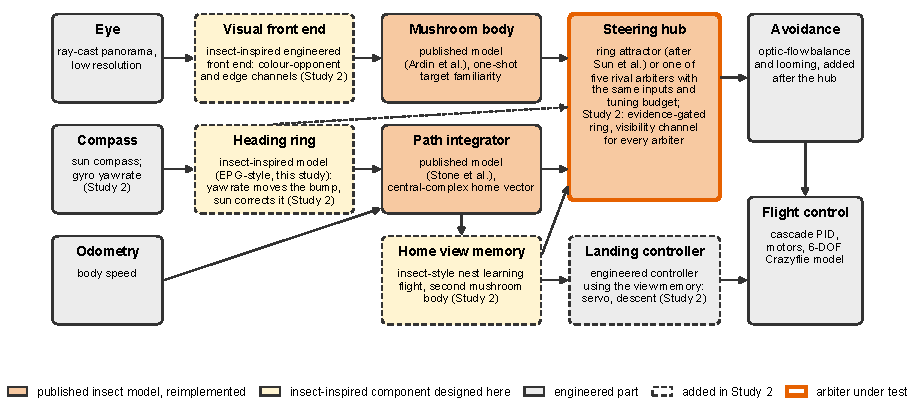
\includegraphics[width=0.92\textwidth]{fig1_system.pdf}
\caption{The controller. Boxes show which part is a reimplemented insect model and which is engineered; dashed boxes were added in Study~2. The steering hub (orange outline) is the part under test: in each arm it is replaced by one of six arbiters that receive the same inputs. Arrows show the main signal flow; the avoidance reflex is added to the hub's heading command.}
\label{fig:system}
\end{figure*}

\subsection{Arbiters and equal-budget tuning}
Six arms replaced the hub in turn: the ring; the ring with recurrence off; a static vote (argmax of the same input stage); a vector sum; a leaky evidence accumulator; and a state machine (search, approach, hold-last-bearing with a timeout, home) written before any fault data and frozen by hash. Its author knew the hypotheses and the fault list. All arms saw, per object, a bearing, a strength and a visibility flag; the state machine used the flag, while the ring and the vote saw only strength times visibility. Every arm received the same 64 configurations drawn from one uniform matrix, evaluated in two rungs on training seeds (3D: all 64 on seeds 0--4, the best 4 on seeds 0--19), and its winner was frozen before any test seed ran. For the ring the budget was equal in number but not in effect: \SoneEnvHighGain{} of the 64 draws had a gain of 0.7 or more, and most of those latched onto their first commitment and never turned home, so only \SoneUsableTwoD{} of 64 were usable in 2D and \SoneUsableThreeD{} of 64 in 3D.

\subsection{Study 1 tests}
\emph{Kill tests (2D point mass).} KT1 (H2) compared the ring's heading with a static vote across two-cue conflicts; KT2 (H1 pilot) flew 28 fault conditions on 300 test seeds; KT3 (H3) measured the hold of a target hidden for 10~s (time until the command leaves its bearing by 20\textdegree, cap 10~s) and the release of a look-alike whose evidence falls below the target's (time from the noise-free crossing until the command reaches the target, cap 20~s), sweeping the ring gain, the accumulator leak and the state-machine timeout with other parameters fixed at their tuned values. \emph{3D mission (H1, H3).} Seven faults at up to four severities gave 25 conditions per seed: target occlusion (1--10~s), a swapped look-alike on the reported spot (similarity 0.5--0.95), a half-silenced compass (one level), dead eye columns (10--40\%), a false sun (30--120\textdegree), a speed-scale error and Dryden gusts. Success required a target stop, a return within 2~m of home and no collision. H1 used test seeds 1000--1299. \emph{Recognition (H4).} MuJoCo renders of a tent and three look-alikes in the target's exact pose, from 0--180\textdegree{} azimuth at three distances, two new suns and camera jitter, on ten test layouts; AUROC of target versus look-alike probes per azimuth.

\subsection{Study 2 modules}
Study~2 was planned after diagnosing Study~1 (Section~\ref{sec:s1}). Every sensory and motor module was given to all six arbiters.
\emph{Heading ring (H5).} An EPG-like ring of 32 neurons whose bump is shifted by the gyro yaw rate and corrected by the sun compass only while their conflict stays inside a tuned gate, with a slow remapping of the cue offset when the conflict persists \citep{seelig2015,kim2017}. Its rivals were a complementary filter and a Kalman filter with a gyro-bias state, each with a gate and the same 64-configuration budget; they were tested on 2D replays of recorded flights (KT5).
\emph{Home view memory and landing (H6).} At take-off the drone flew one outward, rising loop around a striped home pad and stored its views one-shot in a second mushroom body, after insect nest learning flights \citep{philippides2013,collett2018}. On return, once the path integrator placed home within a few metres, the best-matching view locked and a visual vector replaced the home vector. A servo centred the drone over the pad, then it descended at 0.3~m/s to touchdown.
\emph{Visual front end (H8).} Log receptors, a luminance and two colour-opponent channels (an RGB approximation), local contrast normalisation, oriented-edge channels and 6~$\times$~6 pooling on an object-centred crop fed the unchanged mushroom body, after work showing that simple feature detectors support generalisation in a bee-like model \citep{roper2017}. The target learning flight became multi-scale: 30 views at three distances, two heights and three suns (the suns stand for repeated flights at different times of day, an assumption). An inspection rule stopped only after consistent familiarity from two viewpoints at least 20\textdegree{} apart.
\emph{Evidence-gated ring (H7).} The ring's recurrent gain drops when the input away from the bump exceeds the input at it, and hidden objects keep their last evidence, decaying with a tuned time constant; neuromodulation of recurrent synapses has been proposed to set how well bump-attractor memories resist distractors \citep{compte2000}. Every rival received the matching visibility channel. KT7 repeated KT3 with a third trial that penalises premature switching.
\emph{Variable altitude.} The drone searched at \StwoAltSearch{}~m (chosen on training seeds between 2.5 and 3.5~m), descended to inspect a close candidate, climbed to return and descended to land.

\subsection{Study 2 mission (H9)}
Success now required a target stop, touchdown within 0.5~m of the pad centre and no collision within 300~s. The six arbiters were retuned on the Study~2 stack with the same budget (training seeds 100--104, then the best 4 on 100--119). The test ran \StwoNarms{} arms on test seeds 2000--2299 that had never been used: the six arbiters, the Study~1 brain, a Kalman-heading variant, one ablation per module, a 0~s learning flight, and two operator-tip sensitivity arms (no tip, with an outward spiral search; a poor tip of 30\textdegree{} and 30\%). H9 required (i) fault-free success $\geq 0.90$, (ii) an AUC at least 0.15 above the Study~1 brain, and (iii) success $\geq 0.50$ for every fault at its middle severity.

\subsection{Pre-registration and statistics}
For each seed and fault, success was integrated over severity with the trapezoid rule (fault-free run at 0, worst level at 1), and the aggregate AUC is the mean over the seven faults. Differences are paired bootstraps over seeds (10,000 resamples), proportions carry Wilson intervals, and pairwise tests were Holm-corrected. The pre-registered H1 statistic, the ring's AUC minus the largest of the other five, is biased against any arm when arms tie. Amendment~4, made before the 3D test data were reduced and prompted by an independent review, therefore made a within-seed arm-permutation test of that statistic (5,000 permutations) the decision rule; the bootstrap interval is still reported.

\emph{Chronology.} The Study~1 hypotheses were drafted before any data, but the record is an internal log without independent timestamps, and the public commits start after the kill tests and the recognition study. The 3D tuning freeze and Amendment~4 were commits made before the 3D test data were reduced. For Study~2, a SHA-256 hash of the plan was committed before any Study~2 data, and the tuned parameters were committed before any Study~2 test seed ran. Study~2 design choices (search altitude, landing constants, the inspection default) were fixed on training seeds and logged before testing; the component results of H5, H7 and H8 were known before the mission test, which kept the modules as pre-registered. Analyses added after the data are labelled post hoc.

\section{Results}

\subsection{Study 1: the insect parts did not beat the rivals}\label{sec:s1}
\emph{Ring versus vote (H2).} The pre-registered statistic was $D^*=\SoneDstar$\textdegree, above the 5\textdegree{} kill line. Post hoc, it depended on the vote-width grid (\SoneDstarFine--\SoneDstar\textdegree) and fell to \SoneDstarExclLo--\SoneDstarExclHi\textdegree{} without equal-certainty cells, so outside ties H2 sits at the kill line.

\emph{Stubbornness (H3, 2D).} As the ring gain rose from 0, the hold of a hidden target lengthened from \SoneHoldGzero{}~s to at most \SoneHoldMax{}~s and the release of a fading look-alike from \SoneRelGzero{}~s to the 20~s cap from gain \SoneCapGain{} (Fig.~\ref{fig:kt3}a). The accumulator released sooner at the ring's hold at every gain where its frontier was defined (\SoneDaccGone{}~s [\SoneDaccGoneLo, \SoneDaccGoneHi] at gain 0.1, down to \SoneDaccMin{}~s), so the pre-registered claim that the ring's frontier lies above its rivals was rejected. The state machine's zero release is a clamp: unclamped, it switched \SoneSMUnclamped{}~s before the crossing, at an evidence ratio of \SoneSMRatio{}, and no trial penalised early switching. With the ring's other parameters varied (post hoc, training seeds; Fig.~\ref{fig:kt3}b), the best ring configuration held \SoneEnvHold{}~s and released in \SoneEnvRel{}~s, still \SoneEnvDacc{}~s [\SoneEnvDaccLo, \SoneEnvDaccHi] behind the accumulator's envelope. The margin shrank from tens of seconds to about one second but did not reverse.

\begin{figure*}[t]
\centering
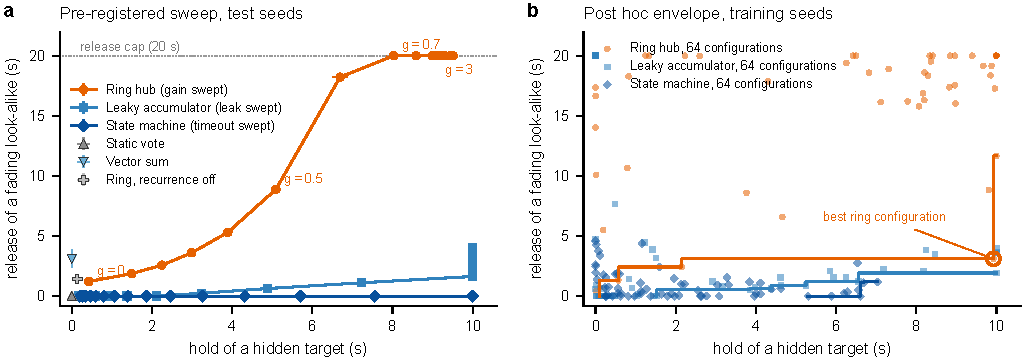
\includegraphics[width=\textwidth]{fig2_kt3.pdf}
\caption{Study~1 stubbornness frontier in the 2D kill test (KT3). (a) Pre-registered sweeps on test seeds (n~=~300 per point): ring gain $g$, accumulator leak time and state-machine timeout, other parameters at their tuned values; single points for the arms without a swept memory. Better is lower right (long hold, fast release). Error bars are $\pm1.96$ standard errors over seeds; release is clamped at 0 and capped at 20~s. (b) Post hoc: all 64 random-search configurations per arm on training seeds 0--99, with each arm's Pareto envelope (lines); the circle marks the ring configuration closest to the accumulator's envelope.}
\label{fig:kt3}
\end{figure*}

\emph{3D mission (H1).} Over \SoneNmissions{} missions on 300 test seeds, the tuned ring (gain \SoneThreeDGain, almost no recurrence) reached an aggregate AUC of \SoneAUCRing{} [\SoneAUCRingLo, \SoneAUCRingHi]; the state machine reached \SoneAUCSM{} and the accumulator \SoneAUCAcc. The pre-registered ring-minus-best-other difference was \SoneHoneDiff{} [\SoneHoneDiffLo, \SoneHoneDiffHi], and the Amendment~4 permutation test gave $p$\,\SoneHonePermP, so H1 held against the ring. The effect was not specific to the ring: post hoc, the vector sum ($p$\,\SoneHoneSumP) and the ring without recurrence ($p$\,\SoneHoneStaticP) failed the same test. The difference came from the swapped look-alike alone (fault AUC ring \SoneDecoyRing, state machine \SoneDecoySM); without that fault all six arms lay between \SoneNoDecoyLo{} and \SoneNoDecoyHi{} (Fig.~\ref{fig:s1mission}). The false sun (\SoneFalseSun), the speed-scale error (\SoneSpeed) and the half compass (\SoneCompass) defeated every arm alike, because arbitration cannot repair a wrong home vector.

\begin{figure*}[t]
\centering
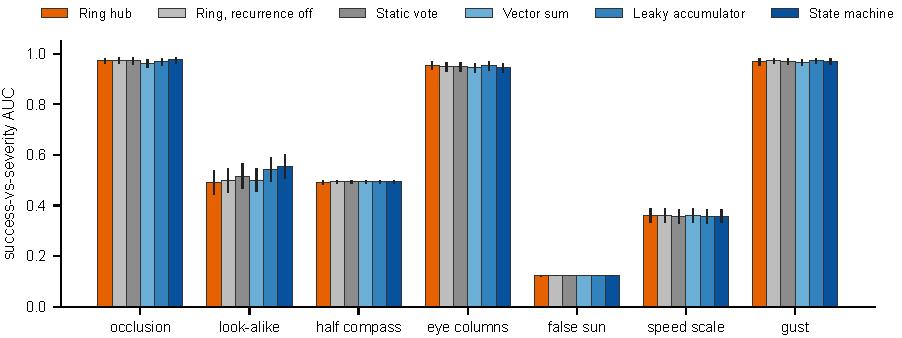
\includegraphics[width=\textwidth]{fig3_s1_mission.pdf}
\caption{Study~1 mission: success-vs-severity AUC per fault for the six arms (test seeds 1000--1299, n~=~300 seeds per arm and condition). Orange, the ring hub; blue, engineered rivals; grey, controls. Error bars are 95\% percentile bootstrap intervals over seeds (10,000 resamples).}
\label{fig:s1mission}
\end{figure*}

\emph{Stubbornness in the mission (H3, 3D).} The pre-registered comparison was inconclusive. The ring's mean hold peaked at \SoneHthreePeak{}~s at gain \SoneHthreePeakGain, and from gain 1 the ring stopped at a hidden target in \SoneHthreeStopGone{} of runs and \SoneHthreeLimitGone{} of runs hit the time limit, so high-gain points describe a latched controller. No arm's mean hold exceeded \SoneHthreeCeil{}~s although the target was hidden for 10~s, because the occlusion began on first sight within 10~m while the drone was closing (a ceiling of the metric). At gain 0 the ring's input stage beat the accumulator's frontier by \SoneHthreeAccGzero{}~s [\SoneHthreeAccGzeroLo, \SoneHthreeAccGzeroHi]; recurrence did not add to that.

\emph{Recognition (H4).} At the stored azimuth, pooled over distance, height jitter and two new suns, the mushroom body's AUROC was \SoneMB{} [\SoneMBLo, \SoneMBHi] and raw pixels \SonePix, with or without the learning flight. DINOv2 patch features, given an object-centred memory, reached \SoneDinoOff{} and \SoneDinoOn{} with the learning flight. H4 was rejected for the mushroom body.

\emph{Diagnosis.} Four causes were identified for Study~2: the path integrator trusted a single sun compass and speed signal; landing used the path integrator alone; the recogniser could not separate look-alikes; and the ring's single gain coupled hold and release.

\subsection{Study 2: the integrated brain completed most missions}
\emph{Components.} Across the false-sun and half-compass faults, the heading ring cut the RMS heading error from \StwoHeadVone\textdegree{} with the Study~1 compass to \StwoHeadRing\textdegree{} [\StwoHeadRingLo, \StwoHeadRingHi] and beat the complementary filter (\StwoHeadCF\textdegree), but the Kalman filter did better (\StwoHeadKF\textdegree; Kalman minus ring \StwoHeadKFdiff\textdegree{} [\StwoHeadKFdiffLo, \StwoHeadKFdiffHi]), so H5 was not supported (Fig.~\ref{fig:heading}a). H7 was rejected: once every arm had a visibility channel, the rivals held and released without a trade-off, the gated ring spent \StwoTimeOffLo--\StwoTimeOffHi~s longer off target than the state machine (\StwoSMtimeOff~s) in the premature-switch trial at gains up to 0.7, and in the 2D mission world it scored \StwoKTsevenGated{} against \StwoKTsevenVote{} for the gated vote ($p$\,\StwoKTsevenP). The visual front end lifted the mushroom body from chance (\StwoMBvone{} on the new layouts) to \StwoFront{} [\StwoFrontLo, \StwoFrontHi] at 0\textdegree, \StwoMargin{} [\StwoMarginLo, \StwoMarginHi] above raw pixels, but missed the 0.75 criterion, so H8 failed (Fig.~\ref{fig:recog}). A nearest-neighbour readout of the same features reached \StwoNN{} and DINOv2 \StwoDino{}; outside the flown arc the mushroom body fell below chance (\StwoFrontNinety{} at 90\textdegree), and the multi-scale flight did not beat the single goal view at 0\textdegree{} (\StwoMSvsGoal{} [\StwoMSvsGoalLo, \StwoMSvsGoalHi]).

\begin{figure}[t]
\centering
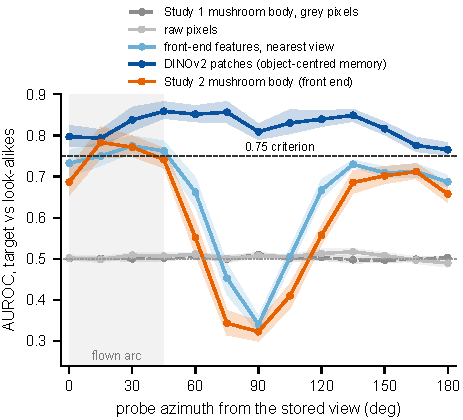
\includegraphics[width=\columnwidth]{fig4_recognition.pdf}
\caption{Recognition under a swap control: AUROC of target versus look-alike probes on the same spot, per 15\textdegree{} azimuth bin (Study~2 test layouts 1010--1019; n~=~120 target and 360 look-alike probes per bin). Memories: the Study~1 learning flight for the Study~1 mushroom body, the multi-scale flight for the others. Bands are 95\% percentile bootstrap intervals over the 10 layouts (2,000 resamples), which likely under-cover with 10 clusters.}
\label{fig:recog}
\end{figure}

\emph{Integrated mission (H9).} In \StwoNmissions{} missions the Study~2 brain completed the full mission in \StwoNoFault{} [\StwoNoFaultLo, \StwoNoFaultHi] of fault-free runs (n~=~\Nseeds), meeting criterion~(i) (Fig.~\ref{fig:headline}). Its aggregate AUC was \StwoAUC{} [\StwoAUCLo, \StwoAUCHi] against \StwoAUCvone{} for the Study~1 brain, which has no landing (difference \StwoDiffVone{} [\StwoDiffVoneLo, \StwoDiffVoneHi]); scored by its own 2~m definition the Study~1 brain reached \StwoVoneOwn{}, still \StwoDiffOwn{} [\StwoDiffOwnLo, \StwoDiffOwnHi] lower. Criterion~(ii) passed. At middle severity, success was \StwoMidOcc{} under occlusion, \StwoMidCompass{} with the half compass, \StwoMidEye{} with dead eye columns, \StwoMidSun{} under a false sun, \StwoMidSpeed{} with a speed-scale error, \StwoMidGust{} in moderate gusts and \StwoMidDecoy{} with a swapped look-alike. Criterion~(iii) failed on the look-alike alone, so H9 was not fully met. Look-alike success stayed between \StwoDecoyLo{} and \StwoDecoyHi{} at every similarity; the drone stopped at the wrong object in \StwoWrongRing{} of all missions (state machine \StwoWrongSM, accumulator \StwoWrongAcc).

\begin{figure*}[t]
\centering
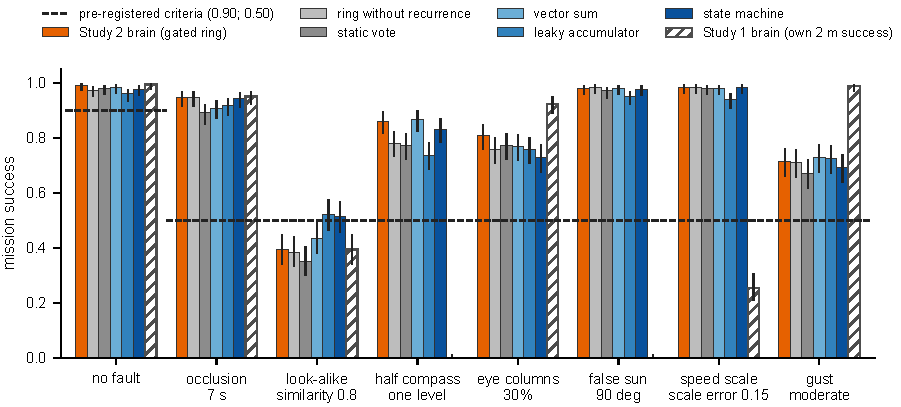
\includegraphics[width=\textwidth]{fig5_s2_headline.pdf}
\caption{Study~2 headline: full-mission success (target stop, touchdown within 0.5~m of the pad, no collision) without faults and at each fault's middle severity, test seeds 2000--2299 (n~=~300 per bar). Orange, the Study~2 brain; blue and grey, the other arbiters on the same Study~2 stack; hatched, the Study~1 brain scored by its own success definition (return within 2~m of home), shown for reference only. Dashed lines are the pre-registered criteria (i) and (iii). Error bars are Wilson 95\% intervals.}
\label{fig:headline}
\end{figure*}

\emph{Arbitration.} With the Study~2 stack, the arbiter barely mattered. The tuned gated ring (gain \StwoTunedGain) scored \StwoAUC; the five rivals ranged from \StwoRivalLo{} to \StwoRivalHi{} (state machine \StwoAUCsm), and the permutation test of ring minus best other gave $p$\,\StwoPermP. Pairwise, only the static vote was lower than the ring after Holm correction (\StwoVsVote, $p$\,\StwoVsVoteP).

\emph{Ablations.} Removing the home view memory cost \StwoAblHome{} AUC [\StwoAblHomeLo, \StwoAblHomeHi], the largest effect of any insect-inspired module (Fig.~\ref{fig:ablation}). Removing the landing controller cost \StwoAblLanding, which is definitional because success requires a touchdown on the pad. Replacing the heading ring with the Study~1 compass cost \StwoAblHeading{} [\StwoAblHeadingLo, \StwoAblHeadingHi]. The front end (\StwoAblFront) and the evidence gating (\StwoAblGated) added little, and the inspection rule nothing (\StwoAblInspect{} [\StwoAblInspectLo, \StwoAblInspectHi]). In the closed loop, the heading ring beat the Kalman variant by \StwoRingMinusKF{} [\StwoRingMinusKFLo, \StwoRingMinusKFHi], the reverse of the 2D replay ranking (Fig.~\ref{fig:heading}b); we did not analyse why.

\begin{figure}[t]
\centering
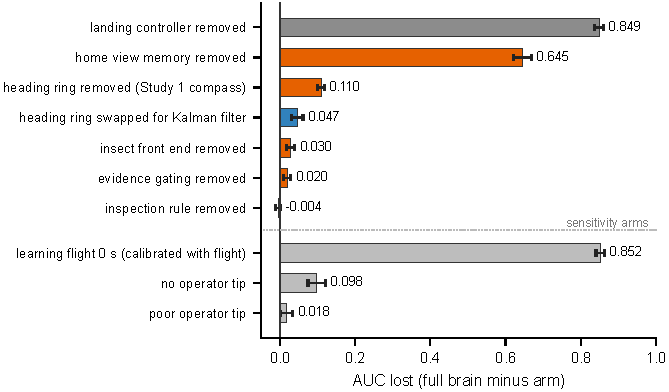
\includegraphics[width=\columnwidth]{fig6_s2_ablations.pdf}
\caption{Study~2 ablations: aggregate AUC of the full brain minus each arm (n~=~300 paired seeds). Orange, insect-inspired modules; blue, the Kalman heading swap; grey, engineered parts; light grey, sensitivity arms. Error bars are 95\% paired bootstrap intervals (10,000 resamples). The landing ablation is definitional, and the 0~s learning flight used an evidence mapping calibrated with learning-flight memories.}
\label{fig:ablation}
\end{figure}

\emph{Sensitivity arms.} With a 0~s learning flight the drone made \StwoLFzeroStops{} target stops in 300 fault-free missions (AUC \StwoLFzero) and collided in \StwoLFzeroColl{} of all runs. Its evidence mapping had been calibrated with learning-flight memories, so this arm tests the calibrated design without its flight, not a design built for a single photo. Without an operator tip the AUC fell to \StwoNoTip{} (fault-free \StwoNoTipNoFault); with a poor tip it was \StwoPoorTip{} (fault-free \StwoPoorTipNoFault).

\emph{Landing (H6).} Fault-free touchdowns had a median error of \StwoLandErr{}~m and a median touchdown speed of \StwoTouch{}~m/s, the descent set-point (Fig.~\ref{fig:landing}). In gusts, \StwoGustPad{} of runs landed on the pad (median error \StwoGustErr{}~m). With the path integrator alone, \StwoPIPad{} of fault-free runs landed on the pad (median error \StwoPIErr{}~m), so the home view memory raised the landing rate as H6 predicted.

\begin{figure*}[t]
\centering
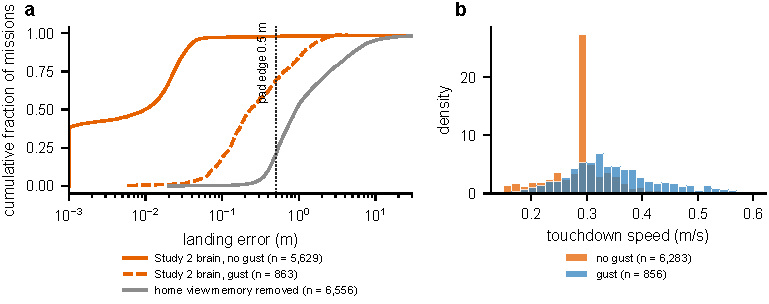
\includegraphics[width=0.78\textwidth]{fig7_landing.pdf}
\caption{Landing in the Study~2 mission (test seeds 2000--2299, all fault conditions). (a) Cumulative distribution of horizontal landing error for missions with a target stop; errors below 1~mm are drawn at 1~mm; the dotted line is the pad edge. (b) Touchdown speed of all touchdowns of the Study~2 brain, split by gusts; the descent set-point is 0.3~m/s. Sample sizes are in the legends.}
\label{fig:landing}
\end{figure*}

\begin{figure*}[t]
\centering
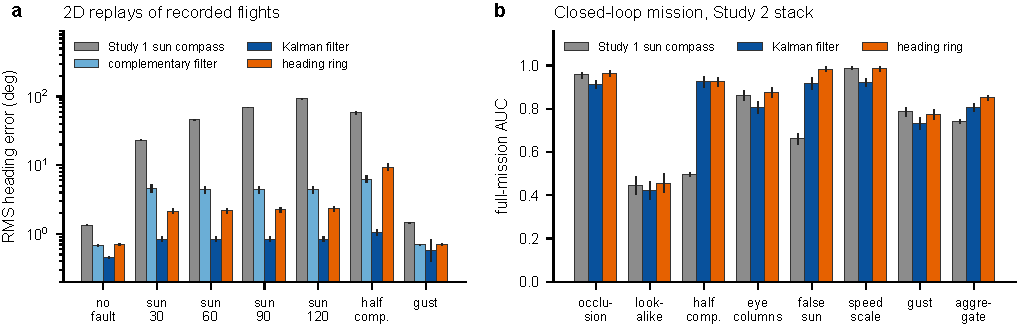
\includegraphics[width=\textwidth]{fig8_heading.pdf}
\caption{Heading estimation. (a) RMS heading error in 2D replays of 300 recorded test flights per condition (KT5; sun offsets in degrees), log scale; error bars are 95\% paired bootstrap intervals (10,000 resamples). (b) Full-mission AUC on the Study~2 stack with the heading ring, the Kalman filter, or the Study~1 sun compass (n~=~300 seeds); error bars are 95\% percentile bootstrap intervals over seeds (10,000 resamples).}
\label{fig:heading}
\end{figure*}

\section{Discussion}

\emph{What worked.} The largest gain came from closing the loop at home. A home view memory loaded during a take-off learning flight and consulted only at the end of the home vector turned path-integrator landings (median error \StwoPIErr{}~m without faults) into touchdowns within centimetres (median \StwoLandErr{}~m), and it absorbed the odometry errors that defeated every Study~1 arm. This matches the role given to nest learning flights in insects \citep{philippides2013,collett2018} and the engineering results of Bee-Nav and AntFlie \citep{beenav2026,antflie2026}. The heading ring was the second contributor: integrating the yaw rate and gating the sun cue largely removed the false-sun and half-compass failures (Fig.~\ref{fig:heading}b). A standard Kalman filter did better in replays and worse in the closed loop, so neither ranking should be read as a property of the insect design.

\emph{What failed.} Look-alike discrimination did not improve enough. The inspection rule did not lower look-alike acceptance in renders, and success with a swapped look-alike stayed near \StwoMidDecoy{} at every similarity. The recognition gain of the front end was real in renders but too small for the stop rule. DINOv2 was the only recogniser above the criterion, with an object-centred memory and a far larger pretrained model.

\emph{Arbitration hardly matters.} In both studies the choice of steering arbiter changed aggregate success little (Study~1: \SoneAUCRing{} to \SoneAUCSM; Study~2: \StwoRivalLo{} to \StwoRivalHi, gated ring \StwoAUC). In Study~1, recurrence traded hold against release, as attractor theory predicts \citep{zhang1996,compte2000}, but rivals with separate knobs did better on both, and the tuner chose almost no recurrence. In Study~2 the rivals reached the same success once they shared the visibility channel and the sensory stack. A ring hub is a workable arbiter for this task; on these data it is not a better one.

\emph{Limitations.} Everything is simulation, and results describe these models in this simulator, not insects or real drones. The modules are published insect models and engineered glue, not connectomes. Optic flow is computed geometrically from ray-casts, and the mission eye is an analytic ray-cast panorama, while the recognition study used MuJoCo renders; object ranges are noise-free. The kill tests are two-dimensional point-mass worlds. Both missions used a single forest world at one obstacle density. In Study~1 the tuning budget was nominal for the ring, the state machine alone used the visibility flag, and the hold metric in 3D saturated far below the 10~s occlusion. The 0~s learning-flight arm inherits an evidence mapping calibrated with flights. Recognition intervals come from 10 layouts and likely under-cover. Two faults in Study~1 were at zero success at every severity, so their weight in the aggregate carries no arm information. Provenance has gaps: early Study~1 result files were stamped with commits that did not yet hold their scripts (later re-stamped and re-run where cheap), the Study~1 pre-registration is not independently timestamped, and Study~2 run records carry no commit because the cloud runs used an archive of the freeze commit; the summary records a SHA-256 hash of every simulation script, and the simulation code is identical at the freeze and results commits.

\section{Conclusion}
In this simulator, insect-model steering hubs did not beat equal-budget engineered rivals, and the mushroom body did not recognise a look-alike on the target's spot. A second, pre-registered design that added an insect-style heading ring and, above all, a nest learning flight with view-based landing completed \StwoNoFault{} of fault-free missions and most faulted ones. It still failed when a look-alike stood where the target was expected.

\section*{Data and code availability}
Code, result files and run records are in the repository \url{https://github.com/aryawidjaja/mutant-brain-drone} (private at the time of writing). Key commits: Study~1 3D tuning freeze \texttt{de9b1e7}; Amendment~4 \texttt{3f8a0cd}; Study~2 plan hash \texttt{3601ce5}; Study~2 tuning freeze \texttt{6c831c7}; Study~2 test results \texttt{ab1e676}. Every result number in this paper is written by \texttt{scripts/export\_compact\_paper.py} from \texttt{results/}, with its source in \texttt{numbers\_sources.json}; the script's self-check re-reads every source and recomputes the main intervals from the run records.

\section*{Acknowledgements and licences}
MuJoCo (Apache-2.0) and the MuJoCo Menagerie Crazyflie model (MIT) \citep{mujoco2012,menagerie2022}; vehicle constants from Förster \citep{forster2015} and Landry \citep{landry2015}, cross-checked against the Crazyflie firmware (GPL-3.0; constants read, no code copied) \citep{cffirmware}. The ring follows Sun, Yue and Mangan; their toolkit is MIT-licensed and was not copied \citep{suntoolkit2024}. The path integrator was reimplemented from the text of Stone and colleagues, whose code has no licence. DINOv2 ViT-S/14 weights (Apache-2.0) \citep{dinov22023}; three.js (MIT) \citep{threejs2026}. No funding was received. The author declares no competing interests.

\section*{AI assistance}
AI coding and writing assistants were used for implementation and drafting; the author reviewed all code, results and text.

\small\raggedright
\bibliographystyle{unsrtnat}
\bibliography{references}

\end{document}
